% relatorio_cho2020.tex: a reproducao de Cho (2020) no NeoPZ (Projects/Cho2020), Passo 1 (a analise deterministica).
% Figuras e tabelas: gera_dados.py, com os dados de ~/projects/runs/cho2020/passo1; ./gera.sh refaz tudo.
\documentclass[11pt,a4paper]{article}
\usepackage[utf8]{inputenc}
\usepackage[T1]{fontenc}
\usepackage[brazil]{babel}
\usepackage{lmodern,amsmath,amssymb,booktabs,graphicx,geometry,caption,float,xcolor}
\usepackage[hidelinks]{hyperref}
\geometry{margin=2.3cm}
\captionsetup{font=small}
\emergencystretch=2em
\providecommand{\versao}{}
\newcommand{\afazer}[1]{\textcolor{red}{[A FAZER: #1]}}

\title{Reprodução de Cho (2020): talude infinito com rocha rasa sob chuva constante\\
\large relatório das simulações (\texttt{Projects/Cho2020}), Passo 1: a análise determinística}
\author{Diogo Cecílio}
\date{\versao}

\begin{document}
\maketitle

\begin{abstract}
S.~E.~Cho (2020), \emph{Failure distribution analysis of shallow landslides under rainfall infiltration based on
fragility curves} (Landslides 17:79--91), deriva curvas de fragilidade de um talude infinito com rocha impermeável
rasa a partir de um modelo de infiltração de Green--Ampt modificado e do FS do talude infinito. Aqui a parte
determinística do artigo (Figs.~3 e 4) é refeita com o Richards do NeoPZ na coluna normal ao talude do Kang2020. O tempo
em que a frente de molhamento chega à rocha, que é o tempo da ruptura, e o FS antes e depois batem com o artigo.
\end{abstract}

\tableofcontents

\section{O problema}
Talude infinito a $\beta = 30^\circ$ com a rocha impermeável a $D = 2$~m na vertical ($L = D\cos\beta = 1{,}732$~m na
normal). O nível d'água inicial está na rocha e o estado inicial é hidrostático: $p_w = -\gamma_w (L - z^*)\cos\beta$,
com $z^*$ a profundidade normal (sucção de 14,7~kPa na superfície). Chuva constante $p$ de $0{,}1$ a $1{,}2\,k_s$. O FS
é a Eq.~21 do artigo,
\[
F_s = \frac{c' + (W\cos^2\beta - \sigma^s)\tan\phi'}{W\sin\beta\cos\beta},\qquad \sigma^s = S_e\,u_w \ (u_w < 0),\quad
\sigma^s = u_w \ (u_w \geq 0),
\]
o mínimo ao longo da profundidade, com $W$ o peso da coluna vertical acima do plano.

\begin{table}[H]\centering\small
\caption{Cho (2020): os valores médios das Tabelas 1 e 2 (a análise determinística).}
\begin{tabular}{lc}
\toprule
$\theta_s$ (= porosidade) / $\theta_r$ & 0,355 / 0\\
van Genuchten: $\alpha$ (1/kPa); $n$ ($m = 1 - 1/n$) & 0,410; 1,120\\
$k_s$ & $1{,}0\times10^{-5}$~m/s (3,6~cm/h)\\
$k_r$ & Mualem\\
$\gamma_d$ (kN/m$^3$); $c'$ (kPa); $\phi'$ ($^\circ$); $\beta$ ($^\circ$) & 17,01; 5; 35; 30\\
\bottomrule
\end{tabular}
\end{table}

\section{O modelo no NeoPZ: a coluna normal ao talude}
O artigo calcula a infiltração com um Green--Ampt modificado (Cho 2017). Aqui ela é o Richards do NeoPZ (o material
$u$--$p_w$--$p_a$ da biblioteca, com o esqueleto rígido e o ar passivo, a variante iii) na coluna normal ao talude, a
mesma do Passo~7 do Kang2020:
\begin{itemize}
  \item a coluna tem a altura normal $L$, 80 células (2,2~cm), cada uma em 4 triângulos; $p_w$ linear (2090 equações);
  \item a gravidade ao longo dela é $g\cos\beta$: a componente paralela não muda as pressões no talude infinito;
  \item a chuva vertical entra como $p\cos\beta$ por metro da superfície inclinada; o excesso escorre (no topo, a chuva
    ou a face de percolação $p_w = 0$); a base (a rocha) é impermeável;
  \item o estado inicial hidrostático com o nível na base sai do \texttt{RainTransient} com $\gamma_w\cos\beta$;
  \item o FS é o \texttt{FSInfinito} do Kang2020 (Eq.~14 do Kang com $p_a = 0$, que é a Eq.~21 do Cho: com
    $\theta_r = 0$, $\chi = S_w = S_e$);
  \item $n = 1{,}12$: o $k_r$ de Mualem tem derivada infinita na saturação, e $k_r$ cai muito rápido com $S_e$. Ele é
    tabelado até $S_e = 1 - \varepsilon$ e fechado suavemente até 1 (\texttt{MualemTabelado.h}). Com
    $\varepsilon = 10^{-3}$ o Newton para quando a frente chega à rocha a partir de $p = 0{,}6\,k_s$; com
    $\varepsilon = 10^{-2}$ ele passa em todas as intensidades (é o que está nas figuras). O preço é pequeno: em
    $p = 0{,}2\,k_s$ a frente chega à rocha em 12,9~h com $\varepsilon = 10^{-2}$ e em 13,2~h com $10^{-3}$.
  \item a frente: o ponto mais fundo em que $S_w$ já subiu metade do que faltava para saturar, na profundidade vertical
    $z^*/\cos\beta$.
\end{itemize}

\section{Resultados}
\begin{table}[H]\centering\small
\caption{O tempo em que a frente chega à rocha (o instante da ruptura) e o FS, NeoPZ e Cho (2020) (lido das Figs.~3 e 4,
$\pm 0{,}2$~h).}\label{tab:tempos}
\begin{tabular}{c|cc|cc|c}
\toprule
$p/k_s$ & \multicolumn{2}{c|}{frente na rocha (h)} & FS inicial & FS final & passos\\
 & NeoPZ & Cho & \multicolumn{2}{c|}{NeoPZ (Cho: 1,50 e 0,92)} & \\
\midrule
0{,}1 & 25{,}30 & 26{,}00 & 1{,}501 & 0{,}914 & 1500\\
0{,}2 & 12{,}90 & 13{,}20 & 1{,}501 & 0{,}914 & 800\\
0{,}3 & 8{,}70 & 8{,}80 & 1{,}501 & 0{,}914 & 1500\\
0{,}4 & 6{,}60 & 6{,}60 & 1{,}501 & 0{,}914 & 802\\
0{,}6 & 4{,}40 & 4{,}40 & 1{,}501 & 0{,}914 & 400\\
0{,}8 & 3{,}40 & 3{,}30 & 1{,}501 & 0{,}914 & 802\\
1{,}0 & 2{,}80 & 2{,}65 & 1{,}501 & 0{,}914 & 800\\
1{,}2 & 2{,}80 & 2{,}50 & 1{,}501 & 0{,}914 & 802\\
\bottomrule
\end{tabular}

\end{table}

\begin{figure}[H]\centering
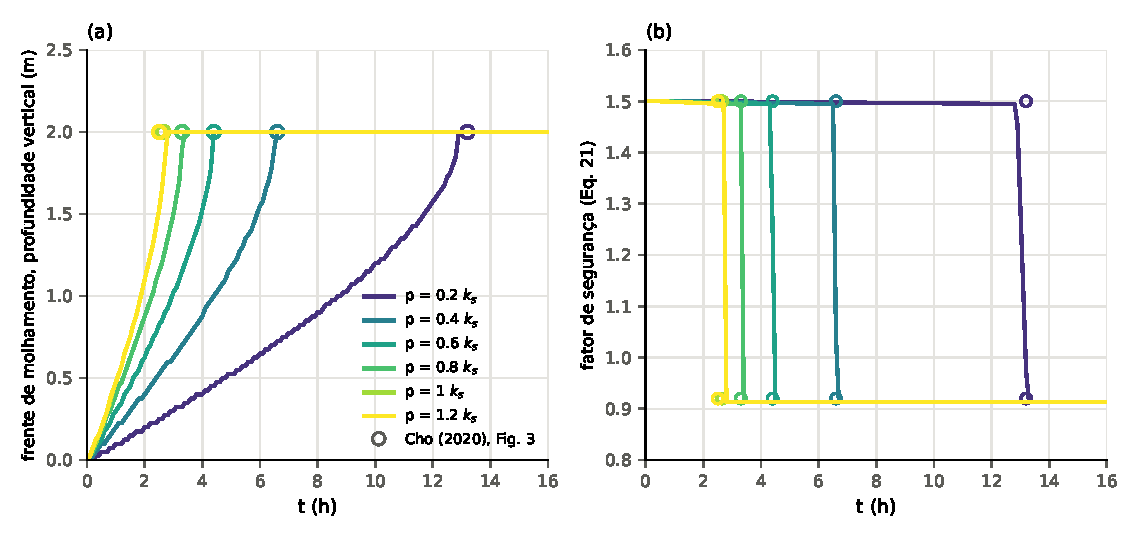
\includegraphics[width=\textwidth]{figs/fig3.pdf}
\caption{(a) A profundidade da frente de molhamento e (b) o FS contra o tempo, NeoPZ (linhas) e Cho (2020) (marcadores:
a frente na rocha, e o FS antes e depois da queda, Fig.~3).}\label{fig:fig3}
\end{figure}

\begin{figure}[H]\centering
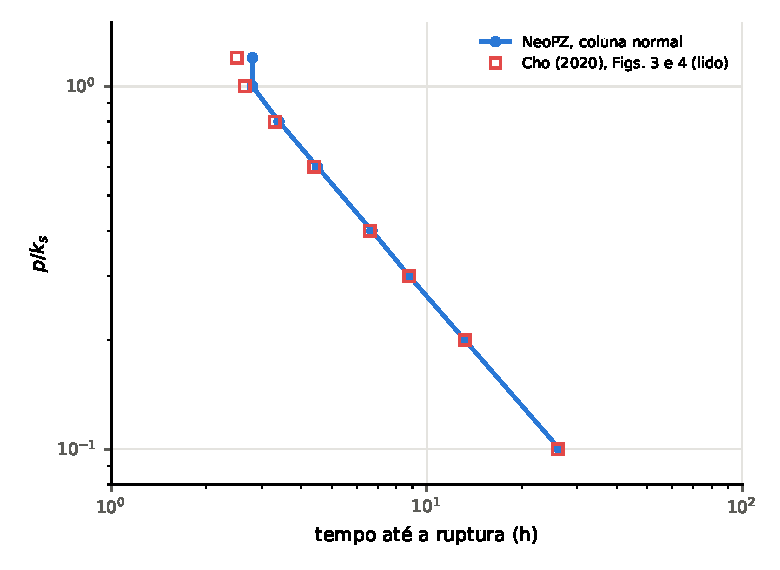
\includegraphics[width=0.7\textwidth]{figs/fig4.pdf}
\caption{A relação intensidade--tempo até a ruptura (o limiar de deflagração determinístico, Fig.~4 do artigo).}
\label{fig:fig4}
\end{figure}

\begin{figure}[H]\centering
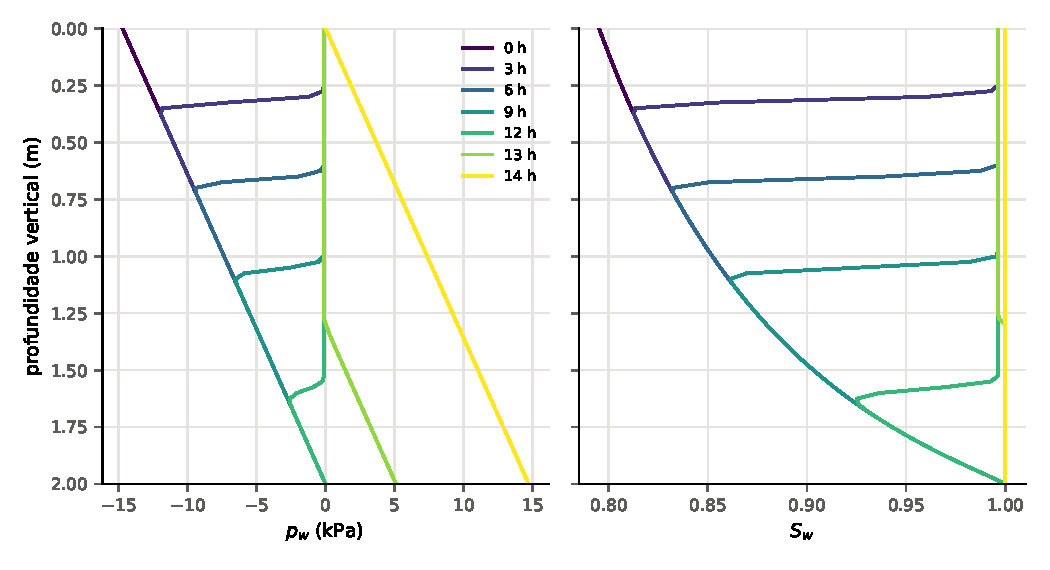
\includegraphics[width=0.85\textwidth]{figs/perfis.pdf}
\caption{Os perfis de $p_w$ e $S_w$ em $p = 0{,}2\,k_s$: a frente desce até a rocha (12,9~h) e, em seguida, a água
se acumula sobre ela e a coluna satura de baixo para cima.}\label{fig:perfis}
\end{figure}

\paragraph{Leitura.} O FS quase não muda enquanto a frente desce (1,501 a 1,495): a frente só tira a sucção da camada
de cima, que não governa a ruptura. Quando ela chega à rocha, a água se acumula sobre a base impermeável, o nível sobe
e a coluna satura toda em minutos, porque com $n = 1{,}12$ o solo já está perto da saturação ($S_w \approx 0{,}8$ a
14,7~kPa) e falta pouca água. O FS cai então de uma vez para 0,914: o talude saturado com escoamento paralelo
($p_w = \gamma_w z\cos^2\beta$), o mesmo do artigo (0,92). O instante da ruptura é o da chegada da frente à rocha, e o
Richards dá os tempos do Green--Ampt modificado do artigo com diferença de até 0,3~h (até 12\,\% em $p = 1{,}2\,k_s$, onde
a chuva já passa da capacidade de infiltração e o tempo depende de como o excesso escorre).

\section{Próximos passos}
\begin{enumerate}
  \item Passo 2: as curvas de fragilidade (Monte Carlo com $k_s$, $\theta_s$, $\alpha$, $n$, $c'$ e $\phi'$
    aleatórios, Tabelas 1 a 3) e a distribuição do tempo de ruptura (lognormal, Eqs.~6 a 13).
  \item O efeito do ar ativo (variante i) na mesma coluna.
\end{enumerate}

\end{document}
